\chapter{Baterai, Sel Bahan Bakar, dan Elektrolisis}\label{ch:b2:batteries-electrolysis}

Setiap kilogram aluminium yang diperoleh dari bijihnya memerlukan sekitar
\qty{13}{kW.h} listrik; melebur satu kilogram skrap, pada prinsipnya, hanya
memerlukan \qty{0.3}{kW.h} untuk memanaskannya sampai titik lebur dan
melelehkannya. Selisihnya adalah kerja sederetan panjang sel \omterm{def:b2:batteries-electrolysis:electrolysis}{elektrolisis},
yang masing-masing mengalirkan ratusan ribu ampere melalui garam cair
pada tegangan beberapa volt. Baterai bekerja ke arah sebaliknya: sebuah
reaksi spontan menggerakkan arus. Dengan \omterm{def:b2:current-potential-curves:ie-curve}{kurva arus--potensial} pada
\cref{ch:b2:current-potential-curves}, keduanya dibaca pada diagram yang
sama, demikian pula sepotong seng yang larut dalam asam.
% ledger: hT:Al_l.933, aw:Al

\begin{recall}
\Cref{ch:b2:cell-thermodynamics}: $\Delta_r G = -nFE$, kerja maksimum,
\omterm{def:b2:cell-thermodynamics:faraday}{tetapan Faraday}. \Cref{ch:b2:current-potential-curves}: \omterm{def:b2:current-potential-curves:ie-curve}{kurva
arus--potensial}, \omterm{def:b2:current-potential-curves:fast-slow}{sistem cepat} dan \omterm{def:b2:current-potential-curves:fast-slow}{sistem lambat}, \omterm{def:b2:current-potential-curves:overpotential}{overpotensial}, \omterm{def:b2:current-potential-curves:limiting-current}{arus
pembatas}, dinding-dinding air. \Cref{ch:b2:ellingham}: mengapa aluminium
tidak diperoleh dengan karbon. Jilid sekolah: \omterm{def:b2:batteries-electrolysis:electrolysis}{elektrolisis}, \omterm{def:b2:batteries-electrolysis:battery}{akumulator}.
\end{recall}

\begin{omfigure}
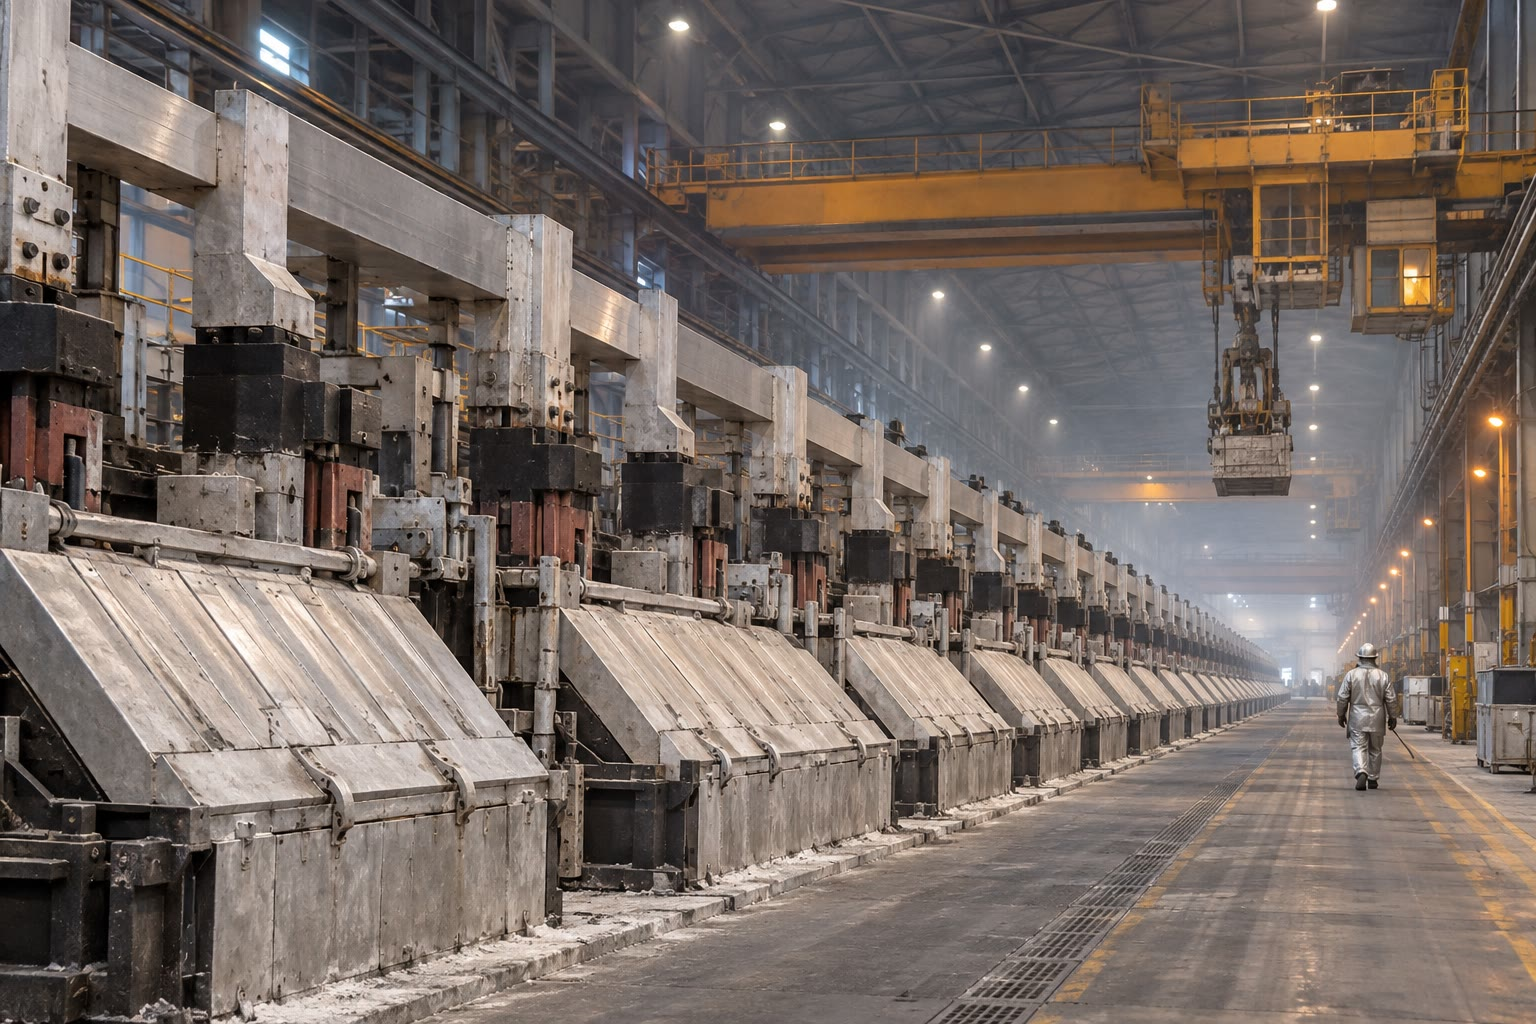
\includegraphics[width=0.62\linewidth]{images/book3/ai/b2-11-potroom.jpg}

{\small Ruang sel sebuah peleburan aluminium: sederet sel \omterm{def:b2:batteries-electrolysis:electrolysis}{elektrolisis},
ratusan banyaknya, yang dihubungkan seri; derek di atasnya mengganti anode
karbon yang habis terbakar.}
\end{omfigure}

\section{Reaksi spontan yang dibaca pada kurva}

\begin{definition}[Potensial campuran]\label{def:b2:batteries-electrolysis:mixed-potential}
Yang disebut \emph{potensial campuran}\index{potensial campuran} sebuah
elektrode tempat dua pasangan berbeda bereaksi, satu dioksidasi dan satu
direduksi, adalah potensial yang diambilnya ketika tidak ada arus bersih
yang mengalir: \omterm{def:b2:current-potential-curves:ie-curve}{arus anodik} satu pasangan lalu sama besar dan berlawanan
arah dengan \omterm{def:b2:current-potential-curves:ie-curve}{arus katodik} pasangan yang lain.
\end{definition}

\begin{proposition}[Logam dalam larutan]\label{prop:b2:batteries-electrolysis:mixed}
Logam yang tercelup dalam larutan yang dapat mengoksidasinya menetap pada
potensial $E_m$ tempat $i_a(E_m) = -i_c(E_m)$, yaitu \omterm{def:b2:current-potential-curves:ie-curve}{arus anodik} oksidasi
logam mengimbangi \omterm{def:b2:current-potential-curves:ie-curve}{arus katodik} reduksi oksidatornya; logam itu larut
dengan laju $i_a(E_m)/(nF)$.
\end{proposition}

\begin{proof}
Sepotong logam yang terisolasi tidak membawa arus bersih. Kedua setengah
reaksi berlangsung di permukaannya pada potensial yang sama, sehingga
arus-arusnya, yang dibaca pada kurva masing-masing pada potensial itu,
berjumlah nol. Menurut \cref{prop:b2:current-potential-curves:current-rate},
\omterm{def:b2:current-potential-curves:ie-curve}{arus anodik} memberikan laju oksidasi.
\end{proof}

\begin{omfigure}
\begin{tikzpicture}
\begin{axis}[omie, width=0.82\linewidth, height=6cm, xmin=-1.1, xmax=-0.3,
  ymin=-3, ymax=3, xlabel={$E$ (V)}, ylabel={$i$}, clip=true, clip mode=individual,
  axis y line=left]
\addplot[omanodic] table[x=E, y=i] {figdata/out/bachelor-2-ie-curves-f-Zn.dat};
\addplot[omcathodic] table[x=E, y=i] {figdata/out/bachelor-2-ie-curves-f-HZn.dat};
\addplot[omcathodic, dashed] table[x=E, y=i] {figdata/out/bachelor-2-ie-curves-f-HCu.dat};
\draw[densely dotted] (axis cs:-0.820,-0.148) -- (axis cs:-0.820,0.148);
\draw[densely dotted] (axis cs:-0.737,-2.38) -- (axis cs:-0.737,2.38);
\fill (axis cs:-0.820,0.148) circle (1.3pt); \fill (axis cs:-0.737,2.38) circle (1.3pt);
\node[font=\scriptsize, anchor=south east] at (axis cs:-0.825,0.2) {seng sendirian};
\node[font=\scriptsize, anchor=west] at (axis cs:-0.73,2.38) {seng menyentuh tembaga};
\node[font=\scriptsize, omThm, anchor=west] at (axis cs:-0.70,1.2) {\ce{Zn} $\to$ \ce{Zn^2+}};
\node[font=\scriptsize, omDef, anchor=north west, align=left] at (axis cs:-0.87,-0.5) {\ce{H+} $\to$ \ce{H2}\\ pada seng};
\node[font=\scriptsize, omDef, anchor=north west] at (axis cs:-0.66,-1.7) {pada tembaga};
\end{axis}
\end{tikzpicture}

{\small Seng dalam asam (kurva model, ion seng encer; potensial dari
$-1.1$ sampai \qty{-0.3}{V}). Jika sendirian, seng menetap pada \omterm{def:b2:batteries-electrolysis:mixed-potential}{potensial
campuran} tempat oksidasinya mengimbangi reduksi \ce{H+} yang lambat pada
seng: arusnya kecil, pelarutannya lambat. Jika menyentuh tembaga, tempat
reduksi \ce{H+} tidak terlalu lambat, keseimbangannya bergeser ke potensial
yang lebih tinggi dan arus yang lebih dari sepuluh kali lebih besar: seng
larut dengan cepat, hidrogen menggelembung pada tembaga.}
\end{omfigure}

Pembacaan yang sama menjelaskan korosi (\cref{ch:b2:corrosion}): laju
korosi sebuah logam adalah arus pada \omterm{def:b2:batteries-electrolysis:mixed-potential}{potensial campurannya}.

\section{Sel yang memberikan arus}

\begin{definition}[Baterai]\label{def:b2:batteries-electrolysis:battery}
Yang disebut \emph{sel primer}\index{sel primer} adalah sel elektrokimia
yang dipakai sekali, sampai pereaksinya habis. Yang disebut
\emph{akumulator}\index{akumulator} adalah sel yang dapat diisi ulang
dengan memaksakan arus melaluinya ke arah sebaliknya, yang membalik
reaksinya. Yang disebut \emph{energi spesifik}\index{energi spesifik}
sebuah sel adalah energi listrik yang diberikannya per satuan massa,
biasanya dalam \unit{W.h/kg}.
\end{definition}

\begin{proposition}[Tegangan sel yang memberikan arus]\label{prop:b2:batteries-electrolysis:delivering}
Sel yang memberikan arus $I$ mempunyai tegangan
\[
  U = E_+ - E_- - \eta_a - |\eta_c| - rI ,
\]
dengan $E_+$ dan $E_-$ potensial kesetimbangan kedua elektrodenya,
$\eta_a > 0$ \omterm{def:b2:current-potential-curves:overpotential}{overpotensial} oksidasi di elektrode negatif, $\eta_c < 0$
\omterm{def:b2:current-potential-curves:overpotential}{overpotensial} reduksi di elektrode positif, dan $r$ hambatan dalam
(elektrolit, separator, sambungan).
\end{proposition}

\begin{proof}
Arus $I$ yang sama bersifat anodik di elektrode negatif, yang potensialnya
dibaca pada kurva anodiknya, $E_- + \eta_a$, dan katodik di elektrode
positif, yang potensialnya $E_+ + \eta_c$. Di antara keduanya, arus
melintasi elektrolit, tempat potensial turun sebesar $rI$. Jadi
$U = (E_+ + \eta_c) - (E_- +
\eta_a) - rI$.
\end{proof}

\begin{omfigure}
\begin{tikzpicture}
\begin{axis}[omie, width=0.82\linewidth, height=5.6cm, xmin=-1.2, xmax=0.8,
  ymin=-2, ymax=2, xlabel={$E$ (V)}, ylabel={$i$}, clip=true, clip mode=individual]
\addplot[omanodic] table[x=E, y=i] {figdata/out/bachelor-2-ie-curves-h-neg.dat};
\addplot[omcathodic] table[x=E, y=i] {figdata/out/bachelor-2-ie-curves-h-pos.dat};
\draw[densely dashed, gray] (axis cs:-1.2,1) -- (axis cs:0.8,1);
\draw[densely dashed, gray] (axis cs:-1.2,-1) -- (axis cs:0.8,-1);
\node[font=\scriptsize, gray, anchor=south west] at (axis cs:-1.18,1) {$+I$};
\node[font=\scriptsize, gray, anchor=north west] at (axis cs:-1.18,-1) {$-I$};
\fill (axis cs:-0.730,1) circle (1.3pt); \fill (axis cs:0.210,-1) circle (1.3pt);
\draw[densely dotted] (axis cs:-0.85,0) -- (axis cs:-0.85,0.5);
\draw[densely dotted] (axis cs:0.45,0) -- (axis cs:0.45,-0.5);
\node[font=\scriptsize, anchor=south] at (axis cs:-0.85,0.5) {$E_-$};
\node[font=\scriptsize, anchor=north] at (axis cs:0.45,-0.5) {$E_+$};
\draw[<->, thick, omProp] (axis cs:-0.730,1.5) -- (axis cs:0.210,1.5) node[midway, above, font=\scriptsize] {$U + rI$};
\draw[densely dotted] (axis cs:-0.730,1) -- (axis cs:-0.730,1.5);
\draw[densely dotted] (axis cs:0.210,-1) -- (axis cs:0.210,1.5);
\node[font=\scriptsize, omThm, anchor=west] at (axis cs:-0.70,0.6) {elektrode negatif};
\node[font=\scriptsize, omDef, anchor=west] at (axis cs:0.30,-1.5) {elektrode positif};
\end{axis}
\end{tikzpicture}

{\small Titik kerja sebuah sel (kurva model). Pada arus $I$, elektrode
negatif berada pada kurva anodiknya, elektrode positif pada kurva
katodiknya; selisih kedua potensial itu, dikurangi penurunan ohmik $rI$,
adalah tegangan yang diberikan. Tegangan itu turun ketika $I$ bertambah.}
\end{omfigure}

\begin{method}[Titik kerja sel atau elektroliser]\label{met:b2:batteries-electrolysis:operating-point}
\begin{enumerate}
  \item Gambarlah kurva anodik elektrode yang dioksidasi dan kurva katodik
        elektrode yang direduksi.
  \item Untuk arus $I$, bacalah potensial setiap elektrode pada $+I$ pada
        kurva anodik dan pada $-I$ pada kurva katodik.
  \item Selisih kedua potensial itu, dikoreksi dengan $rI$ (dikurangkan
        untuk sel, ditambahkan untuk \omterm{def:b2:batteries-electrolysis:electrolysis}{elektroliser}), adalah tegangannya.
\end{enumerate}
\end{method}

\begin{example}[Aki timbal--asam]\label{ex:b2:batteries-electrolysis:lead}
Di elektrode negatif \ce{Pb + SO4^2- -> PbSO4 + 2e-}; di elektrode positif
\ce{PbO2 + 4H+ + SO4^2- + 2e- -> PbSO4 + 2H2O}. Secara keseluruhan
\[
  \ce{Pb + PbO2 + 4H+ + 2SO4^2- -> 2PbSO4 + 2H2O},
\]
$\Delta_r G^\circ = 2(-813.14) + 2(-237.13) - (-217.33) - 2(-744.53) =
\qty{-394.1}{kJ/mol}$, $E^\circ = 394\,100/(2 \times 96\,485) = \qty{2.04}{V}$.
Kedua elektrode tertutup timbal sulfat ketika sel melepaskan muatan;
pengisian membalik reaksinya. Reduksi \ce{H+} pada timbal dan oksidasi air
pada timbal dioksida berlangsung lambat: itulah sebabnya sel \qty{2}{V}
dapat diisi di dalam air, yang jendela termodinamikanya hanya selebar
\qty{1.23}{V}.
% ledger: dfg:PbSO4_cr, dfg:H2O_l, dfg:PbO2_cr, dfg:SO42-_ao
\end{example}

\begin{omfigure}
\begin{tikzpicture}[font=\small, >={Stealth}]
  \draw[thick] (0,0) rectangle (6,3.2);
  \fill[omDef!10] (0.05,0.05) rectangle (5.95,2.7);
  \fill[black!45] (0.6,0.4) rectangle (1.1,2.9);
  \fill[brown!60!black] (4.9,0.4) rectangle (5.4,2.9);
  \draw[thick] (0.85,2.9) -- (0.85,3.9) node[pos=0.75, left] {$-$};
  \draw[thick] (5.15,2.9) -- (5.15,3.9) node[pos=0.75, right] {$+$};
  \draw[->, thick, omProp] (0.85,3.9) -- (0.85,4.3) -- (5.15,4.3) -- (5.15,3.95);
  \node[font=\scriptsize, omProp, anchor=south] at (3,4.3) {$\mathrm{e^-}$ saat pengosongan};
  \node[font=\scriptsize, align=center] at (0.85,-0.45) {\ce{Pb}\\ (\ce{PbSO4} saat pengosongan)};
  \node[font=\scriptsize, align=center] at (5.15,-0.45) {\ce{PbO2}\\ (\ce{PbSO4} saat pengosongan)};
  \node[font=\scriptsize, align=center] at (3.0,1.6) {larutan \ce{H2SO4}\\ \ce{H+}, \ce{HSO4-}, \ce{SO4^2-}};
\end{tikzpicture}

{\small Aki timbal--asam, skematis. Saat pengosongan, timbal dioksidasi dan
timbal dioksida direduksi, keduanya menjadi timbal sulfat, dan asamnya
terkonsumsi: massa jenis larutan menunjukkan keadaan muatan.}
\end{omfigure}

\begin{omfigure}
\begin{tikzpicture}[font=\small, >={Stealth}]
  \draw[thick] (0,0) rectangle (7,3);
  % graphite layers
  \foreach \y in {0.5,0.9,1.3,1.7,2.1,2.5} \draw[thick, black!70] (0.3,\y) -- (2.3,\y);
  \foreach \y in {0.7,1.1,1.5,1.9,2.3} \foreach \x in {0.6,1.3,2.0} \fill[omDef] (\x,\y) circle (0.07);
  % layered oxide
  \foreach \y in {0.5,0.9,1.3,1.7,2.1,2.5} \draw[thick, omThm] (4.7,\y) -- (6.7,\y);
  \foreach \y in {0.7,1.5,2.3} \foreach \x in {5.0,5.7,6.4} \fill[omDef] (\x,\y) circle (0.07);
  \draw[densely dashed] (3.5,0) -- (3.5,3);
  \node[font=\scriptsize, align=center] at (1.3,-0.45) {grafit (negatif)};
  \node[font=\scriptsize, align=center] at (5.7,-0.45) {oksida berlapis (positif)};
  \node[font=\scriptsize, anchor=south] at (3.5,3.0) {separator};
  \draw[->, thick, omThm] (2.5,2.1) -- (4.5,2.1) node[midway, above, font=\scriptsize, fill=white, inner sep=1pt] {\ce{Li+} saat pengosongan};
  \draw[<-, thick, omDef] (2.5,0.9) -- (4.5,0.9) node[midway, below, font=\scriptsize, fill=white, inner sep=1pt] {\ce{Li+} saat pengisian};
\end{tikzpicture}

{\small Sel litium-ion, skematis. Ion-ion litium (titik biru) berada di
antara lapisan-lapisan grafit dalam sel yang terisi; saat pengosongan,
ion-ion itu melintasi elektrolit untuk menyusup di antara lapisan-lapisan
sebuah oksida logam, sementara elektron mengitari rangkaian luar. Tidak ada
elektrode yang larut atau mengendap: ion-ion itu bolak-balik di antara dua
inang.}
\end{omfigure}

\begin{history}[Tumpukan Volta]
\begin{minipage}[t]{0.27\linewidth}
\vspace{0pt}
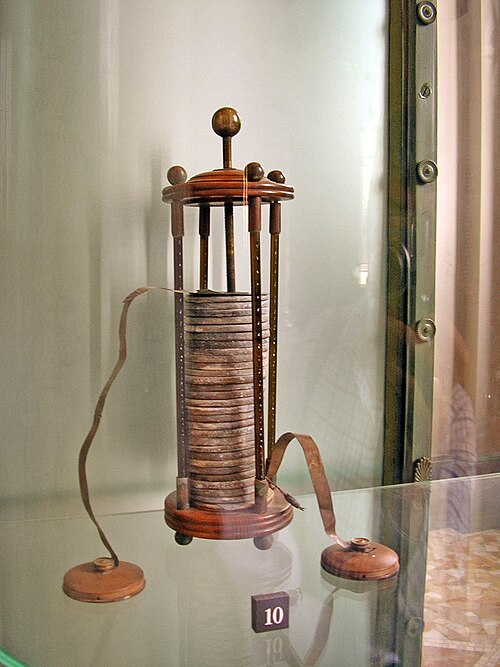
\includegraphics[width=\linewidth]{images/book3/volta-pile.jpg}
\end{minipage}\hfill
\begin{minipage}[t]{0.69\linewidth}
\vspace{0pt}
Pada tahun 1800 Alessandro Volta memerikan sebuah kolom cakram dari dua
logam yang berbeda, seng dan tembaga atau perak, yang dipisahkan oleh kain
yang dibasahi air garam: sumber arus listrik tetap yang pertama. Dalam
beberapa minggu, orang lain memakainya untuk menguraikan air, dan dalam
satu dasawarsa Humphry Davy telah mengisolasi natrium dan kalium dengan
\omterm{def:b2:batteries-electrolysis:electrolysis}{elektrolisis} hidroksidanya yang meleleh memakai tumpukan yang besar. Foto
ini menunjukkan salah satu tumpukan buatan Volta sendiri. (Foto: GuidoB,
CC BY-SA 3.0, Wikimedia Commons.)
\end{minipage}
\end{history}

\section{Sel bahan bakar}

\begin{definition}[Sel bahan bakar]\label{def:b2:batteries-electrolysis:fuel-cell}
Yang disebut \emph{sel bahan bakar}\index{sel bahan bakar} adalah sel yang
pereaksinya, sebuah bahan bakar dan sebuah oksidator (biasanya oksigen
dari udara), diumpankan terus-menerus ke elektrode-elektrodenya dan yang
produknya disingkirkan, sehingga sel itu memberikan arus selama dipasok.
\end{definition}

Dalam sel membran penukar proton pada bus di
\cref{ch:b2:cell-thermodynamics}, hidrogen dioksidasi pada katalis platina,
\ce{H2 -> 2H+ + 2e-}, proton melintasi membran polimer asam yang tipis, dan
oksigen direduksi di sisi yang lain, \ce{O2 + 4H+ + 4e- -> 2H2O}. Oksidasi
hidrogen pada platina adalah \omterm{def:b2:current-potential-curves:fast-slow}{sistem cepat}; reduksi oksigen lambat pada
setiap elektrode. Sebagian besar tegangan yang hilang antara \qty{1.23}{V}
sel reversibel dan tegangan kerjanya adalah \omterm{def:b2:current-potential-curves:overpotential}{overpotensial} elektrode
oksigen, sisanya hambatan membran dan, pada arus tinggi, pasokan oksigen ke
katalis (sebuah \omterm{def:b2:current-potential-curves:limiting-current}{arus pembatas}).

\section{Elektrolisis}

\begin{definition}[Elektrolisis]\label{def:b2:batteries-electrolysis:electrolysis}
Yang disebut \emph{elektrolisis}\index{elektrolisis} adalah reaksi redoks
tak spontan yang dipaksakan oleh arus yang dipasok oleh generator luar; sel
tempat elektrolisis berlangsung disebut
\emph{elektroliser}\index{elektroliser}. Anode, tempat oksidasi terjadi,
dihubungkan dengan kutub positif generator.
\end{definition}

\begin{proposition}[Tegangan minimum termodinamika]\label{prop:b2:batteries-electrolysis:minimum-voltage}
\omterm{def:b2:batteries-electrolysis:electrolysis}{Elektrolisis} yang reaksinya mempunyai $\Delta_r G > 0$ memerlukan
tegangan paling sedikit $\Delta_r G/(nF)$.
\end{proposition}

\begin{proof}
Generator memasok kerja $nFU$ per mol reaksi; menurut
\cref{thm:b2:cell-thermodynamics:delta-g-nfe} yang diterapkan pada reaksi
kebalikannya, kerja listrik yang diterima harus paling sedikit
$\Delta_r G$.
\end{proof}

\begin{proposition}[Tegangan elektroliser]\label{prop:b2:batteries-electrolysis:electrolysis-voltage}
\omterm{def:b2:batteries-electrolysis:electrolysis}{Elektroliser} yang mengalirkan arus $I$ memerlukan
\[
  U = (E_a - E_c) + \eta_a + |\eta_c| + rI ,
\]
dengan $E_a$, $E_c$ potensial kesetimbangan pasangan anode dan katode
($E_a - E_c = \Delta_r G/(nF)$), $\eta_a$, $\eta_c$ \omterm{def:b2:current-potential-curves:overpotential}{overpotensialnya} pada
arus itu, dan $r$ hambatan di antara kedua elektrode.
\end{proposition}

\begin{proof}
Seperti pada sel, arus yang sama bersifat anodik di anode, pada potensial
$E_a +
\eta_a$, dan katodik di katode, pada $E_c + \eta_c$; generator juga
harus mendorongnya melalui elektrolit, yang menambahkan $rI$.
\end{proof}

\begin{method}[Meramalkan elektrolisis]\label{met:b2:batteries-electrolysis:predict-electrolysis}
\begin{enumerate}
  \item Daftarlah setiap spesies yang dapat dioksidasi di anode (termasuk
        logam anode dan pelarutnya) dan setiap spesies yang dapat
        direduksi di katode (termasuk pelarutnya).
  \item Gambarlah \omterm{def:b2:current-potential-curves:ie-curve}{kurva arus--potensialnya} pada bahan-bahan elektrode yang
        dipakai.
  \item Ketika tegangan dinaikkan, kurva anodik pertama dan kurva katodik
        pertama yang tercapai memberikan reaksinya; pada arus yang lebih
        besar, kurva-kurva berikutnya menambahkan reaksinya.
\end{enumerate}
\end{method}

\begin{definition}[Efisiensi faraday]\label{def:b2:batteries-electrolysis:faradaic-efficiency}
Yang disebut \emph{efisiensi faraday}\index{efisiensi faraday} $\eta_F$
sebuah \omterm{def:b2:batteries-electrolysis:electrolysis}{elektrolisis} adalah fraksi muatan yang dialirkan yang menghasilkan
produk yang dikehendaki. Selanjutnya, \emph{konsumsi energi
spesifiknya}\index{konsumsi energi spesifik} adalah energi listrik yang
dipakai per satuan massa produk.
\end{definition}

\begin{proposition}[Hukum Faraday]\label{prop:b2:batteries-electrolysis:faraday-mass}
Arus $I$ yang dialirkan selama waktu $t$ dengan \omterm{def:b2:batteries-electrolysis:faradaic-efficiency}{efisiensi faraday} $\eta_F$
menghasilkan massa $m = \eta_F MIt/(nF)$ produk bermassa molar $M$ yang
dibentuk dengan $n$ elektron per mol.
\end{proposition}

\begin{proof}
Muatan $It$, yang $\eta_F It$ di antaranya membentuk produk, bersesuaian
menurut \cref{prop:b2:cell-thermodynamics:charge} dengan $\eta_F It/(nF)$
mol.
\end{proof}

\begin{proposition}[Energi per kilogram]\label{prop:b2:batteries-electrolysis:energy}
Pada tegangan $U$ dan \omterm{def:b2:batteries-electrolysis:faradaic-efficiency}{efisiensi faraday} $\eta_F$, \omterm{def:b2:batteries-electrolysis:faradaic-efficiency}{konsumsi energi
spesifiknya} adalah $w = nFU/(\eta_F M)$.
\end{proposition}

\begin{proof}
Energinya adalah $UIt$ dan massanya $\eta_F MIt/(nF)$; bagilah.
\end{proof}

\section{Elektrolisis industri}

\paragraph{Seng.} Sebagian besar seng diperoleh dengan \omterm{def:b2:batteries-electrolysis:electrolysis}{elektrolisis} larutan
seng sulfat yang asam pada \cref{ch:b2:ellingham}. Seng diendapkan di katode
walaupun \ce{H+} adalah oksidator yang lebih kuat: pada seng, reduksi
\ce{H+} sangat lambat, dan gelombang seng tercapai lebih dahulu; anode
melepaskan oksigen.

\begin{omfigure}
\begin{tikzpicture}
\begin{axis}[omie, width=0.82\linewidth, height=5.6cm, xmin=-1.6, xmax=2.4,
  ymin=-2.4, ymax=2.4, xlabel={$E$ (V)}, ylabel={$i$}, clip=true, clip mode=individual]
\addplot[omcathodic] table[x=E, y=i] {figdata/out/bachelor-2-ie-curves-g-cath.dat};
\addplot[omanodic] table[x=E, y=i] {figdata/out/bachelor-2-ie-curves-g-an.dat};
\draw[densely dotted] (axis cs:-0.76,-2.2) -- (axis cs:-0.76,0.4);
\draw[densely dotted] (axis cs:0,-2.2) -- (axis cs:0,0.4);
\node[font=\scriptsize, anchor=south] at (axis cs:-0.76,0.4) {$-0.76$};
\node[font=\scriptsize, anchor=south east] at (axis cs:-0.02,0.4) {$0$};
\node[font=\scriptsize, omDef, anchor=north west, align=left] at (axis cs:-0.7,-1.05) {\ce{Zn^2+} $\to$ \ce{Zn},\\ plato};
\node[font=\scriptsize, omDef, anchor=east, align=right] at (axis cs:-1.32,-0.9) {\ce{H+} $\to$ \ce{H2}\\ pada Zn};
\node[font=\scriptsize, omThm, anchor=east] at (axis cs:1.85,1.6) {\ce{H2O} $\to$ \ce{O2}};
\node[font=\scriptsize, gray, align=center] at (axis cs:-0.38,-0.5) {tidak ada \ce{H2}\\ pada seng di sini};
\end{axis}
\end{tikzpicture}

{\small \omterm{def:b2:batteries-electrolysis:electrolysis}{Elektrolisis} larutan seng sulfat yang asam dengan katode seng (kurva
model). Walaupun pasangan \ce{H+}/\ce{H2} ($\qty{0}{V}$) terletak di atas
\ce{Zn^2+}/\ce{Zn} ($\qty{-0.76}{V}$), reduksi \ce{H+} pada seng baru
dimulai sekitar \qty{-1.1}{V}: di antaranya, hanya seng yang diendapkan. Di
anode, air dioksidasi menjadi oksigen.}
\end{omfigure}

\paragraph{Klor dan natrium hidroksida.} Air garam pekat dielektrolisis di
dalam sel yang dibagi oleh membran yang hanya dapat dilewati kation. Di
anode, klorida dioksidasi, \ce{2Cl- -> Cl2 + 2e-}; di katode, air direduksi,
\ce{2H2O +
2e- -> H2 + 2OH-}; ion-ion natrium melintasi membran untuk
menyeimbangkan muatan, dan larutan natrium hidroksida yang bebas klorida
keluar dari sisi katode. Tegangan minimum termodinamikanya adalah
$\Delta_r G/(2F) = \qty{2.19}{V}$ untuk \ce{2Cl- + 2H2O -> Cl2 +
H2 + 2OH-}
dalam kondisi standar. Klor terbentuk di anode alih-alih oksigen, walaupun
pasangan \ce{O2}/\ce{H2O} terletak lebih rendah: oksidasi air adalah yang
lebih lambat di antara keduanya pada bahan-bahan anode yang dipakai.
% ledger: dfg:OH-_ao, dfg:Cl-_ao, dfg:H2O_l

\begin{omfigure}
\begin{tikzpicture}[font=\small, >={Stealth}]
  \draw[thick] (0,0) rectangle (6,3.4);
  \draw[thick, dashed, omProp] (3,0) -- (3,3.4);
  \fill[black!30] (0.4,0.3) rectangle (0.7,3.0);
  \fill[black!50] (5.3,0.3) rectangle (5.6,3.0);
  \node[font=\scriptsize] at (0.55,3.3) {$+$};
  \node[font=\scriptsize] at (5.45,3.3) {$-$};
  \node[font=\scriptsize, align=center] at (1.85,1.9) {air garam\\ \ce{2Cl-} $\to$\\ \ce{Cl2 + 2e-}};
  \node[font=\scriptsize, align=center] at (4.2,1.9) {larutan\\ \ce{NaOH}\\ \ce{2H2O + 2e-} $\to$\\ \ce{H2 + 2OH-}};
  \draw[->, thick, omDef] (2.6,0.8) -- (3.4,0.8) node[pos=0.1, above, font=\scriptsize] {\ce{Na+}};
  \draw[->, thick] (1.0,3.4) -- (1.0,4.0) node[above] {\ce{Cl2}};
  \draw[->, thick] (5.0,3.4) -- (5.0,4.0) node[above] {\ce{H2}};
  \draw[->, thick] (-0.8,0.6) -- (0,0.6) node[pos=0, left] {air garam masuk};
  \draw[->, thick] (6,0.6) -- (6.8,0.6) node[right] {\ce{NaOH} keluar};
  \node[font=\scriptsize, omProp, anchor=north] at (3,-0.05) {membran penukar kation};
\end{tikzpicture}

{\small Sel kloralkali membran, skematis. Hanya ion natrium yang melintasi
membran, sehingga hidroksida yang terbentuk di katode tidak bertemu dengan
klor.}
\end{omfigure}

\paragraph{Aluminium.} Aluminium oksida dilarutkan dalam kriolit cair,
\ce{Na3AlF6}, yang melebur jauh lebih rendah daripada alumina, lalu
dielektrolisis di antara katode karbon, tempat aluminium cair terkumpul,
dan anode-anode karbon yang terbakar habis menjadi karbon dioksida (proses
Hall--Héroult):
\[
  \ce{2Al2O3 + 3C -> 4Al + 3CO2} .
\]
Tegangan minimum termodinamikanya di dekat \qty{1250}{K} sekitar
\qty{1.18}{V} (\cref{pb:b2:batteries-electrolysis:1}); sel pada soal itu
bekerja pada tiga setengah kali nilai itu, dan kelebihannya diubah menjadi
kalor yang menjaga bak tetap cair.

\begin{omfigure}
\begin{tikzpicture}[font=\small, >={Stealth}]
  \draw[thick, fill=black!12] (0,0) rectangle (7,3.2);
  \fill[black!45] (0.3,0.3) rectangle (6.7,0.8);
  \fill[gray!35] (0.3,0.8) rectangle (6.7,1.4);
  \fill[orange!30] (0.3,1.4) rectangle (6.7,2.5);
  \foreach \x in {1.0,3.0,5.0} {
    \fill[black!75] (\x,1.75) rectangle (\x+1.0,3.6);
    \draw[thick] (\x+0.5,3.6) -- (\x+0.5,4.2);
  }
  \draw[thick] (1.5,4.2) -- (5.5,4.2) node[right] {$+$};
  \node[font=\scriptsize, align=left, anchor=west] at (7.3,2.6) {anode karbon, terbakar menjadi \ce{CO2}};
  \node[font=\scriptsize, align=left, anchor=west] at (7.3,1.95) {kriolit cair + \ce{Al2O3} terlarut};
  \node[font=\scriptsize, align=left, anchor=west] at (7.3,1.1) {aluminium cair (katode)};
  \node[font=\scriptsize, align=left, anchor=west] at (7.3,0.55) {blok katode karbon, $-$};
  \draw[densely dotted] (6.7,2.6) -- (7.3,2.6) (6.7,1.95) -- (7.3,1.95) (6.7,1.1) -- (7.3,1.1) (6.7,0.55) -- (7.3,0.55);
\end{tikzpicture}

{\small Sel Hall--Héroult, penampang, skematis. Aluminium direduksi di
permukaan kolam logam cair, yang berperan sebagai katode; ion-ion oksida
dilepaskan pada anode-anode karbon, yang dibakarnya menjadi karbon
dioksida.}
\end{omfigure}

\begin{history}[Hall dan Héroult, 1886]
\begin{minipage}[t]{0.18\linewidth}
\vspace{0pt}
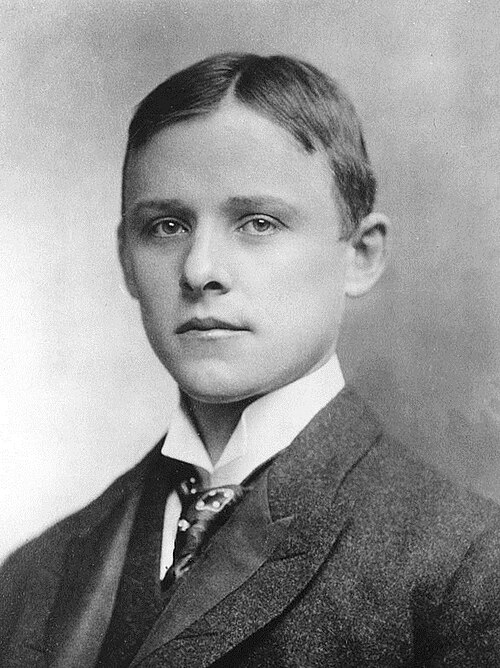
\includegraphics[width=\linewidth]{images/book3/hall.jpg}
\end{minipage}\hspace{0.02\linewidth}%
\begin{minipage}[t]{0.18\linewidth}
\vspace{0pt}
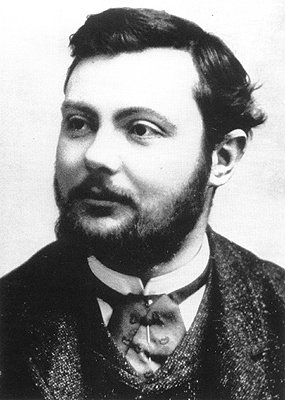
\includegraphics[width=\linewidth]{images/book3/heroult.jpg}
\end{minipage}\hfill
\begin{minipage}[t]{0.58\linewidth}
\vspace{0pt}
Pada tahun 1886, pada usia dua puluh dua atau dua puluh tiga tahun,
Charles Martin Hall dan Paul Héroult, di dua sisi Samudra Atlantik,
menemukan secara terpisah bahwa alumina larut dalam kriolit cair dan dapat
dielektrolisis di sana. Aluminium, yang sampai saat itu merupakan logam
berharga yang dibuat dengan mereduksi kloridanya dengan natrium, menjadi
logam ringan yang paling murah begitu listrik dapat dibangkitkan dalam
jumlah besar. (Potret: Hall, sekitar tahun 1880-an, penulis tidak
diketahui, domain publik; Héroult, domain publik; Wikimedia Commons.)
\end{minipage}
\end{history}

\paragraph{Natrium.} Natrium tidak dapat diendapkan dari air, yang
direduksinya. Natrium dibuat dengan \omterm{def:b2:batteries-electrolysis:electrolysis}{elektrolisis} natrium klorida cair, yang
titik leburnya diturunkan oleh garam tambahan (\omterm{def:b2:solid-liquid-diagrams:eutectic}{campuran eutektik},
\cref{ch:b2:solid-liquid-diagrams}), dengan klor sebagai produk samping.
Pada \qty{1100}{K}, $\Delta_f G^\circ(\ce{NaCl}, \text{l}) =
\qty{-310.7}{kJ/mol}$: tegangan minimumnya \qty{3.22}{V}.
% ledger: janafG:NaCl.1100

\section{Latihan}

\begin{exercise}[$\star$]\label{exo:b2:batteries-electrolysis:1}
Pada gambar seng dalam asam, bacalah \omterm{def:b2:batteries-electrolysis:mixed-potential}{potensial campuran} dan arus seng
sendirian dan seng yang menyentuh tembaga (satuan model), lalu nyatakan
mana yang larut lebih cepat.
\end{exercise}

\begin{exercise}[$\star$]\label{exo:b2:batteries-electrolysis:2}
Berapa massa seng yang diendapkan dalam satu jam oleh arus \qty{500}{A}
dengan \omterm{def:b2:batteries-electrolysis:faradaic-efficiency}{efisiensi faraday} 100~\%?
\end{exercise}

\begin{exercise}[$\star$]\label{exo:b2:batteries-electrolysis:3}
Hitunglah tegangan standar aki timbal--asam dari \omterm{def:b2:reaction-free-energy:gibbs-energy}{energi Gibbs} pembentukan
yang diberikan dalam bab ini, serta jumlah sel dalam aki mobil
\qty{12}{V}.
\end{exercise}

\begin{exercise}[$\star$]\label{exo:b2:batteries-electrolysis:4}
Berapa muatan, dalam ampere-jam, yang dapat diberikan oleh satu gram
litium jika seluruhnya dioksidasi menjadi \ce{Li+}?
\end{exercise}

\begin{exercise}[$\star\star$]\label{exo:b2:batteries-electrolysis:5}
Sebuah sel pemurnian tembaga mengalirkan \qty{200}{A} selama \qty{24}{h}
dan mengendapkan \qty{5.50}{kg} tembaga. Hitunglah \omterm{def:b2:batteries-electrolysis:faradaic-efficiency}{efisiensi faraday-nya}.
\end{exercise}

\begin{exercise}[$\star\star$]\label{exo:b2:batteries-electrolysis:6}
Sebuah sel \omterm{def:b2:batteries-electrolysis:electrolysis}{elektrolisis} pengambilan seng bekerja pada \qty{3.3}{V} dengan
\omterm{def:b2:batteries-electrolysis:faradaic-efficiency}{efisiensi faraday} 90~\% (data latihan). Hitunglah energi listrik per
kilogram seng.
\end{exercise}

\begin{exercise}[$\star\star$]\label{exo:b2:batteries-electrolysis:7}
Sebuah baterai memberikan \qty{1.55}{V} pada \qty{0.10}{A} dan
\qty{1.40}{V} pada \qty{0.60}{A}. Dengan menganggap \omterm{def:b2:current-potential-curves:overpotential}{overpotensialnya} dapat
diabaikan, tentukan hambatan dalamnya dan tegangannya tanpa arus.
\end{exercise}

\begin{exercise}[$\star\star$]\label{exo:b2:batteries-electrolysis:8}
Air garam pekat dielektrolisis di dalam sel membran. Tuliskan reaksi-reaksi
elektrodenya, hitunglah tegangan minimumnya, lalu jelaskan mengapa
produk-produknya harus dijaga terpisah.
\end{exercise}

\begin{exercise}[$\star\star$]\label{exo:b2:batteries-electrolysis:9}
Hitunglah tegangan minimum \omterm{def:b2:batteries-electrolysis:electrolysis}{elektrolisis} natrium klorida cair pada
\qty{1100}{K} dan energi minimum per kilogram natrium.
\end{exercise}

\begin{exercise}[$\star\star\star$]\label{exo:b2:batteries-electrolysis:10}
Dengan \omterm{def:b2:current-potential-curves:ie-curve}{kurva arus--potensial}, jelaskan mengapa seng dapat dilapiskan dari
bak asam pada katode seng, lalu ramalkan apa yang akan terjadi pada katode
platina pada awal pelapisan.
\end{exercise}

\begin{exercise}[$\star\star\star$]\label{exo:b2:batteries-electrolysis:11}
Dari $\Delta_f G^\circ$ pada \qty{1100}{K} dan \qty{1300}{K} ($\ce{Al2O3}$:
$-1328.3$ dan $-1262.3$; $\ce{CO2}$: $-396.0$ dan $-396.2$ \unit{kJ/mol}),
hitunglah tegangan minimum sel Hall--Héroult pada \qty{1250}{K}, lalu
bandingkan dengan anode inert tempat oksigen akan dilepaskan.
\end{exercise}

\begin{exercise}[$\star\star\star$]\label{exo:b2:batteries-electrolysis:12}
Listrik disimpan dengan mengelektrolisis air pada \qty{1.80}{V} dan
diperoleh kembali dalam \omterm{def:b2:batteries-electrolysis:fuel-cell}{sel bahan bakar} pada \qty{0.70}{V}, keduanya dengan
\omterm{def:b2:batteries-electrolysis:faradaic-efficiency}{efisiensi faraday} 100~\%. Hitunglah efisiensi bolak-baliknya dan jelaskan
ke mana energinya pergi.
\end{exercise}

\section{Soal: Satu Ton Aluminium}

\begin{problem}[{Soal akhir pekan --- reaksi sel Hall--Héroult dan tegangan
minimumnya, muatan dan waktu untuk membuat satu ton aluminium, energi yang
dipakai, dan karbon yang terbakar}]
\label{pb:b2:batteries-electrolysis:1}
Data: \omterm{def:b2:reaction-free-energy:gibbs-energy}{energi Gibbs} pembentukan JANAF pada \qty{1100}{K} dan \qty{1300}{K}
(\unit{kJ/mol}): \ce{Al2O3} $-1328.3$, $-1262.3$; \ce{CO2} $-396.0$,
$-396.2$. Sel (data latihan): arus \qty{300}{kA}, tegangan \qty{4.1}{V},
\omterm{def:b2:batteries-electrolysis:faradaic-efficiency}{efisiensi faraday} 94~\%, bak di dekat \qty{1250}{K}. Massa molar
(\unit{g/mol}): Al 26.982, C 12.011, O 15.999. Kalor untuk membawa
aluminium dari \qty{298}{K} sampai cair pada titik leburnya:
\qty{28.69}{kJ/mol}.
% ledger: janafG:Al2O3.1100, janafG:Al2O3.1300, janafG:CO2.1100, janafG:CO2.1300, aw:Al, aw:C, aw:O, hT:Al_l.933, const:F

\medskip
\noindent\textbf{Bagian I --- Tegangan minimum.}
\begin{enumerate}
  \item Berikan bilangan oksidasi aluminium, oksigen, dan karbon dalam
        pereaksi dan produk.
  \item Tuliskan setengah reaksi katode dan anode, dengan ion oksida
        \ce{O^2-} yang dibawa oleh bak cair.
  \item Tuliskan reaksi keseluruhan dan jumlah $n$ elektron yang
        dipertukarkan.
  \item Interpolasikan $\Delta_f G^\circ$ \ce{Al2O3} dan \ce{CO2} pada
        \qty{1250}{K}.
  \item Hitunglah $\Delta_r G^\circ$ pada \qty{1250}{K}.
  \item Simpulkan tegangan minimumnya.
  \item Hitunglah tegangan minimum dengan anode inert,
        \ce{2Al2O3 -> 4Al + 3O2}, lalu jelaskan peran karbon.
\end{enumerate}

\medskip
\noindent\textbf{Bagian II --- Muatan dan waktu.}
\begin{enumerate}[resume]
  \item Berapa jumlah zat aluminium dalam satu ton?
  \item Berapa muatan yang diperlukan dengan \omterm{def:b2:batteries-electrolysis:faradaic-efficiency}{efisiensi faraday} 100~\%?
  \item Berapa muatan yang sebenarnya dialirkan?
  \item Berapa lama waktu yang diperlukan satu sel untuk membuat satu ton?
  \item Berapa massa aluminium yang dibuat satu sel per hari?
  \item Usulkan ke mana perginya 6~\% muatan yang hilang.
\end{enumerate}

\medskip
\noindent\textbf{Bagian III --- Energi.}
\begin{enumerate}[resume]
  \item Hitunglah energi listrik per ton.
  \item Nyatakan energi itu dalam \unit{kW.h} per kilogram.
  \item Hitunglah energi minimum per kilogram, pada tegangan minimum dan
        efisiensi 100~\%.
  \item Ke mana perginya sisa energi itu, dan mengapa energi itu tidak
        sepenuhnya terbuang?
  \item Hitunglah daya listrik satu sel.
  \item Hitunglah kalor yang diperlukan untuk melebur kembali satu kilogram
        skrap, dalam \unit{kW.h}, lalu bandingkan.
  \item Berapa bagian tegangan kerja yang merupakan minimum termodinamika?
\end{enumerate}

\medskip
\noindent\textbf{Bagian IV --- Karbon.}
\begin{enumerate}[resume]
  \item Hitunglah massa karbon yang terbakar per ton aluminium menurut
        persamaannya.
  \item Hitunglah massa karbon dioksida yang dilepaskan oleh anode per ton.
  \item Sel nyata membakar lebih banyak karbon daripada itu. Usulkan dua
        alasannya.
  \item Nyatakan \ce{CO2} dari anode per kilogram aluminium.
  \item Apa yang akan diubah oleh anode inert pada tegangan dan pada gas
        yang dilepaskan?
  \item Nyatakan energi listrik per kilogram aluminium.
\end{enumerate}
\end{problem}
